%卒論中間審査用研究概要テンプレート ver. 1.0

\documentclass[uplatex,twocolumn]{jsarticle}
\usepackage[top=22mm,bottom=22mm,left=20mm,right=20mm]{geometry}
\setlength{\columnsep}{15mm}
\usepackage[T1]{fontenc}
\usepackage{txfonts}
\usepackage{wrapfig}
\usepackage[expert,deluxe]{otf}
\usepackage[dvipdfmx,hiresbb]{graphicx}
\usepackage[dvipdfmx]{hyperref}
\usepackage{pxjahyper}
\usepackage{secdot}

\makeatletter
\renewcommand{\section}{\@startsection{section}{1}{\z@}{0pt}{0.4\Cvs}{\normalfont\raggedright}}
\renewcommand{\subsection}{\@startsection{subsection}{2}{\z@}{\z@}{\z@}{\normalfont}}
\renewcommand{\subsubsection}{\@startsection{subsubsection}{3}{\z@}{\z@}{\z@}{\normalfont}}
\makeatother
%ここから上を編集する必要はない.





%タイトルと学生番号,名前だけ編集すること
\title{\vspace{-5mm}\fontsize{14pt}{0pt}\selectfont クラウドファンディングにおける成功の判別分析}
\author{\normalsize プロジェクトマネジメントコース・ソフトウェア開発管理グループ 矢吹研究室 1242105 三浦泰介}
\date{}
\pagestyle{empty}
\begin{document}
\fontsize{10.5pt}{\baselineskip}\selectfont
\maketitle





%以下が本文
\section{研究の背景}
\makeatletter\renewcommand{\section}{\@startsection{section}{1}{\z@}{0.6\Cvs}{0.4\Cvs}{\normalfont\raggedright}}\makeatother%余白の調整(気にしなくていい)

クラウドファンディング\cite{wiki}と呼ばれる資金調達の手法が世界中で流行りを見せており,その波は日本にも来ている.クラウドファンディングとは,プロジェクトの活動資金を,インターネットを利用し,不特定多数の支援者から募集する資金調達の手法であり,個人規模の小さなプロジェクトでも利用できるため,近年ベンチャー企業や学生から注目を集めている.クラウドファンディングは一般的に資金提供者に対するリターンの形態によって以下の3つに分けることができる.
\begin{description}
 \item[寄付型] 金銭的リターンのない
 \item[投資型] 金銭的リターンのある
 \item[購入型] 権利や物品を購入することで支援する
\end{description}
日本では金融商品取引法\cite{keizai}が2014年に改正されるまで,法規制の問題から,見返りを得ない寄付型,購入型に限られていた.購入型はリターンがあるためリターンを目当てに多くの出資者が集まる傾向があり,購入型は日本で一番市場が大きいクラウドファンディングの形態である.今回は市場が,最も大きい購入型のプロジェクトの成功率に関わる成功要因を探すこととする.


\section{目的}

クラウドファンディングサイトに掲載されているプロジェクトから,支援の金額,コースの数など支援者側から見える情報をデータとして集め,決定木を描くことで,クラウドファンディングにおける成功要因を明らかにし,クラウドファンディングを用いたプロジェクトを行う際や投資する際の参考となる指標を作ることを目的とする.

\section{研究方法}

クラウドファンディングサイトを,毎日定時に監視し,データを収集を行う.プロジェクトの内容や代表者から知り得る情報を元に判別分析を行い,成功要因を考察する,成功合否の判別を行い,実際の合否との一致率を上げることで信憑性を確保する.

\section{成果物のイメージ}

プロジェクトの情報からクラウドファンディングの合否を決定する決定木を書くこと.プロジェクトの成功予測を8割以上で行えるようにすることを成果物の目標とする.
\begin{figure}[h]
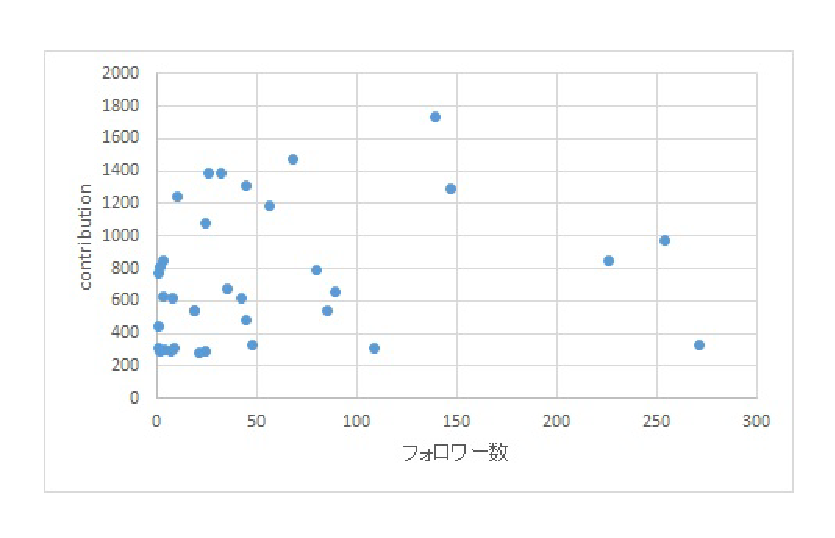
\includegraphics[width=7cm,clip]{figure.pdf}
\caption{決定木}\label{サンプル図}
\end{figure}

\section{進捗状況}

一ヶ月分の監視データを集め終えた.サイトごとにフォーマットが違うデータを処理するため,各サイトごとにある情報を確認し,成功要因と思わしき情報を一つのファイルにまとめる方法を模索している.その間も随時データを集め続け可能な限り多くのデータを用いて判別分析を行う.

\section{今後の計画}

これまでに集めたデータを解析し,決定木を書くことでクラウドファンディングの成功要因を明らかにする.成功予測を行い,実際の結果と成功よ予測の結果の的中率を8割以上に上げることの二点を目標に分析を続ける.





\bibliographystyle{junsrt}
\bibliography{biblio}%「biblio.bib」というファイルが必要.

\end{document}
